\begin{figure}[H]
    \caption{Sistema de colores de los modelos}
    \centering
    \setlength{\tabcolsep}{0pt}
    \renewcommand{\arraystretch}{1.2}
    \begin{tabular}{
        |>{\centering\arraybackslash}m{(\textwidth - 4\arrayrulewidth) / 3}
        |>{\centering\arraybackslash}m{(\textwidth - 4\arrayrulewidth) / 3}
        |>{\centering\arraybackslash}m{(\textwidth - 4\arrayrulewidth) / 3}|
    }
        \hline

        \vspace{2pt}
        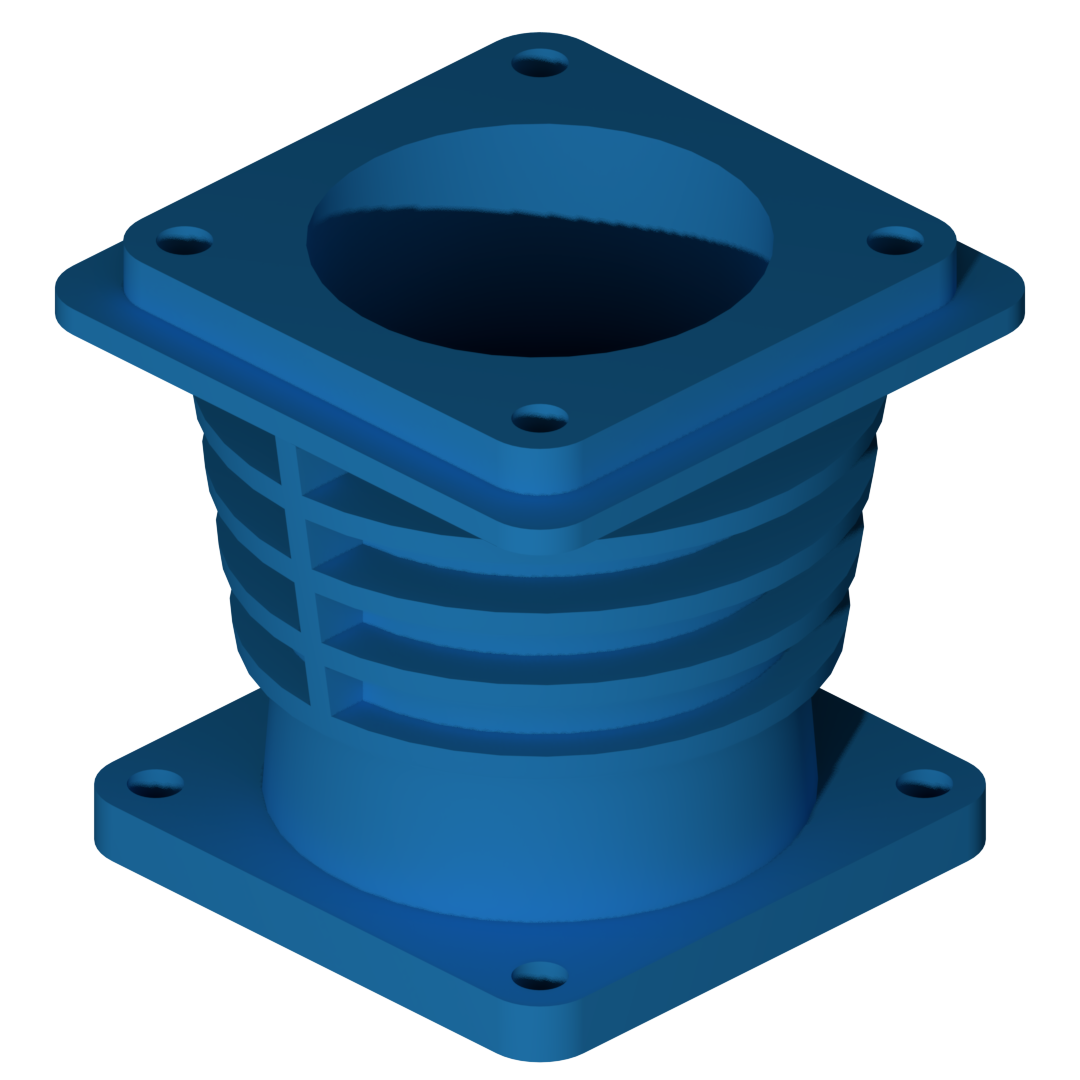
\includegraphics[width=0.33\textwidth]
        {assets/figures/second_phase/img_model_unselected_color.png} &
            \vspace{2pt}
            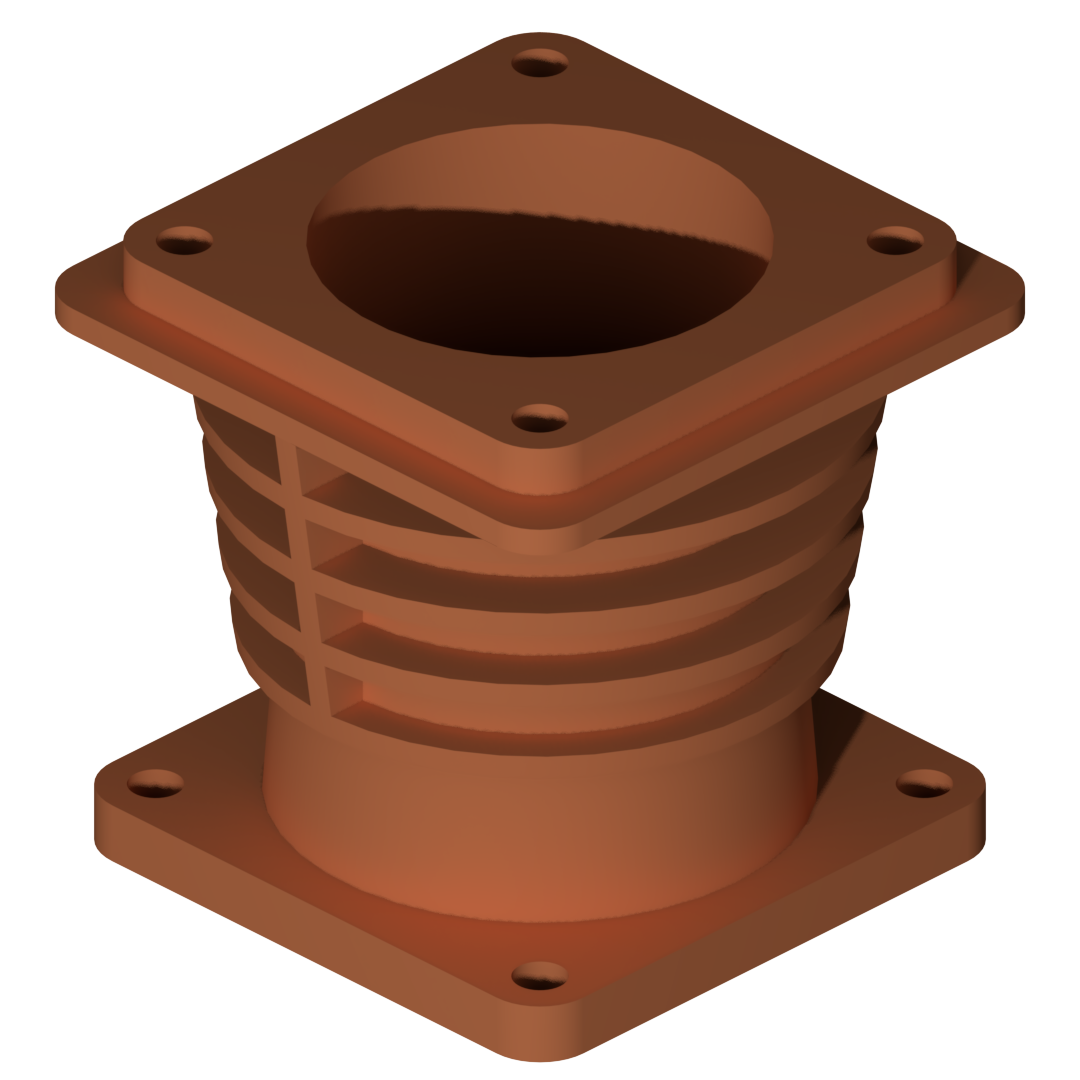
\includegraphics[width=0.33\textwidth]
        {assets/figures/second_phase/img_model_selected_color.png} &
                \vspace{2pt}
                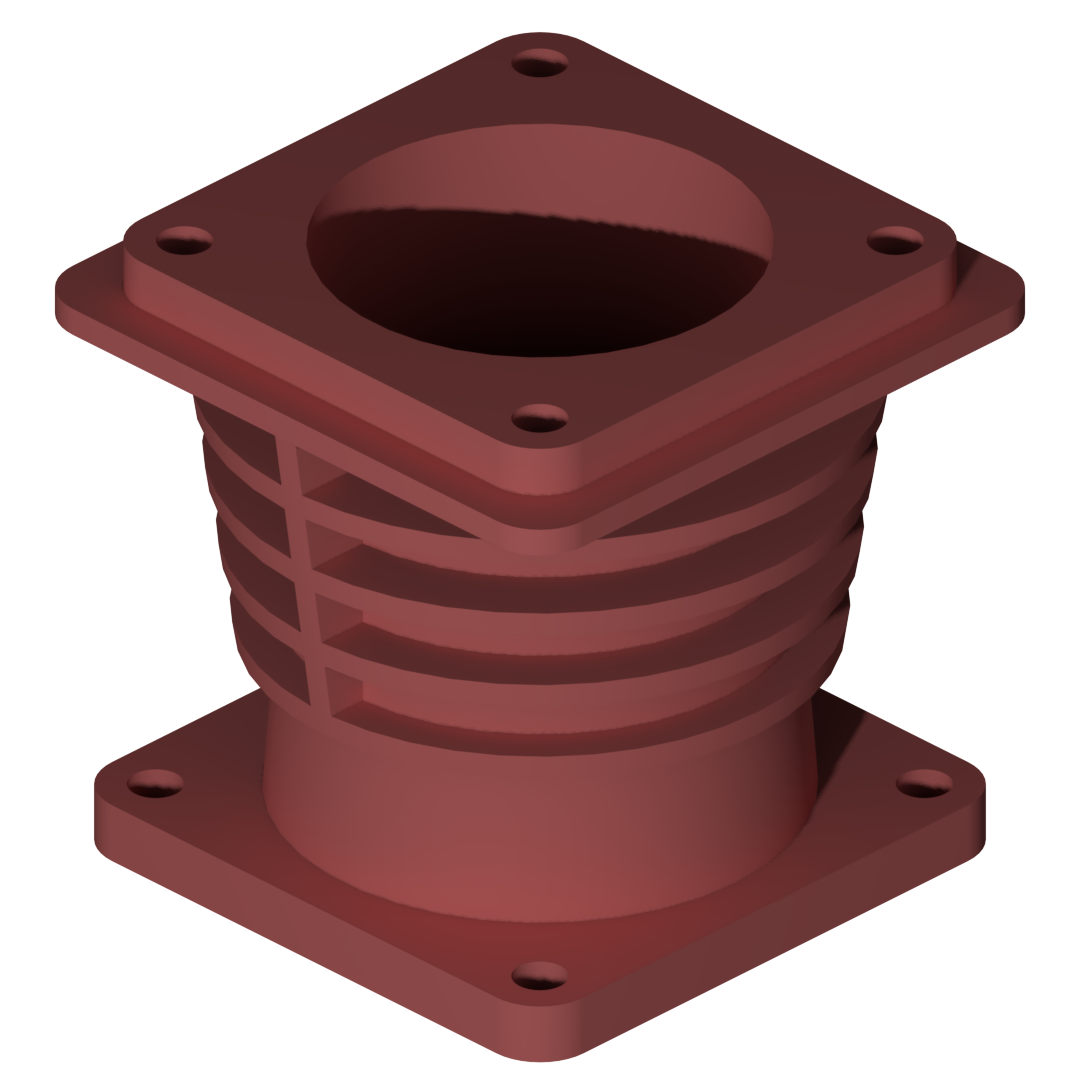
\includegraphics[width=0.31\textwidth]
        {assets/figures/second_phase/img_model_playing_color.png} \\

        \rule{0pt}{0.6cm}\small Estado base &
            \rule{0pt}{0.6cm}\small Estado de selección &
                    \rule{0pt}{0.6cm}\small Estado de animación \\
        
        \hline
    \end{tabular}
    \label{fig:models_colors}
\end{figure}
\fixvspace{0}